%===============================================================================
%   CLASSE ET PACKAGES                                                         %
%========================                                                      %
%	\documentclass[12pt,oneside,french,a4paper]{article} % twoside             %
	\documentclass[conference]{IEEEtran}                                       %
%===============================================================================
%	\usepackage{amsfonts}		% Ens. Math. : $\mathbb{R}$ = ens. des réels   %
	\usepackage{amsmath}		% Mathématiques                                %
	\usepackage{amssymb}		% Symbols, grec ; O pour la complexité : $\mathcal{O}$
%	\usepackage{array}			% Tableaux                                     %
%	\usepackage[french]{babel}	% Français                                     %
	\usepackage[english]{babel}	% Anglais                                      %
	\usepackage{booktabs}		% Tableaux pro                                 %
	\usepackage{cite}			% Recommandé pour IEEEtran                     %
	\usepackage{color}			% Pour utiliser les couleurs                   %
%	\usepackage{eurosym}		% Symbole Euro (\euro)                         %
%	\usepackage{fancybox}		% Cadres                                       %
%	\usepackage{fancyhdr}		% En-têtes, pieds de page                      %
	\usepackage{float}			% Gestion des flottants ([H] <-> HERE.)        %
	\usepackage{flushend}		% Équilibre les colonnes (\raggedend désactive)%
%	\usepackage[left=2cm, top=2cm, right=2cm, bottom=2cm]{geometry}	% Dimensions
	\usepackage{graphicx}		% Inclusion graphiques                         %
%	\usepackage{listings}		% Listings de code                             %
%	\usepackage{multicol}		% Édition sur plusieurs colonnes               %
%	\usepackage{multirow}		% Cellules tableaux sur plusieurs lignes       %
%	\usepackage{numprint}		% Nombres avec espacements (\numprint{+-4,5e6,7})
%	\usepackage{pdfpages}		% Inclusion de PDF                             %
%	\usepackage{setspace}		% Gestion interlignes                          %
%	\usepackage[normalem]{ulem}	% \uline \uuline \uwave \sout \xout \(dash|dot)uline
	\usepackage{xcolor}			% Texte en couleur                             %
	\usepackage{xspace}			% Espaces après macros                         %
%	\usepackage{hyperref}		% Liens hypertextes                            %
%===============================================================================
	\begingroup\expandafter\expandafter\expandafter\endgroup                   %
	\expandafter\ifx\csname directlua\endcsname\relax	% compilé avec LuaTeX ?%
%		\usepackage{lmodern}		% Fontes                                   %
%		\usepackage{mathptmx}		% Fontes Adobe Times Roman                 %
%		\usepackage{mathrsfs}		% Fontes amstex                            %
		\usepackage[utf8]{inputenc}	% Encodage                                 %
		\usepackage[T1]{fontenc}	% Encodage : T1 = Norme Latex (mais != par défaut)
	\else                                                                      %
%		\usepackage{luatextra}				% Paquet pour LuaTeX               %
%		\defaultfontfeatures{Ligatures=TeX}	% Conserver les ligatures          %
%		\setmainfont{Linux Libertine O}
%		\setsansfont{Linux Biolinum O}
%		\setmonofont{}
	\fi                                                                        %
%===============================================================================
%   OPTIONS, COULEURS, MACROS                                                  %
%=============================                                                 %
%	\hypersetup{                                                               %
%		linktoc=all,                                                           %
%		breaklinks,                                                            %
%		colorlinks,                                                            %
%		linkcolor=black,                                                       %
%		citecolor=black,                                                       %
%		urlcolor=blue,                                                         %
%		baseurl       = http://,                                               %
%		pdfpagelayout = OneColumn, % pdfpagelayout=SinglePage                  %
%		pdfstartpage  = 1,                                                     %
%		pdfcreator    = {\LaTeX{}},                                            %
%		pdfproducer   = {\LaTeX{}},% Contient automatiquement le compilateur   %
%		bookmarksopen = true,                                                  %
%		bookmarksdepth= 2,% montrer les sections et sous-sections              %
%		pdfauthor     = {Quentin MONNET, Lynda MOKDAD, Jalel BEN-OTHMAN},
%		pdftitle      = {Energy-balancing method to detect denial of service attacks in wireless sensor networks},
%		pdfsubject    = {A new algorithm for control nodes selection submitted to ICC 2014},
%		pdfkeywords   = {Wireless sensor networks; Reliability, availability, and serviceability; Energy-aware systems; Simulation}
%	}                                                                          %
%===============================================================================
	\definecolor{vert}{rgb}{0.11,0.47,0.11}                                    %
	\newcommand\apriori{\textit{a~priori}\xspace}                              %
	\newcommand\aposteriori{\textit{a~posteriori}\xspace}                      %
	\newcommand\defacto{\textit{de~facto}\xspace}                              %
	\newcommand\eg{\textit{e.g.}\xspace}                                       %
	\newcommand\ie{\textit{i.e.}\xspace}                                       %
	\newcommand\via{\textit{via}\xspace}                                       %
	\newcommand\etc{\textit{et~cætera}\xspace}                                 %
	\newcommand\Wsns{Wireless sensor networks\xspace}                          %
	\newcommand\wsns{wireless sensor networks\xspace}                          %
	\newcommand\Wsn{Wireless sensor network\xspace}                            %
	\newcommand\wsn{wireless sensor network\xspace}                            %
	\newcommand\dos{denial of service\xspace}                                  %
	\newcommand\bs{base station\xspace}                                        %
	\newcommand\BS{BS\xspace}			                                       %
	\newcommand\ch{cluster head\xspace}                                        %
	\newcommand\chs{cluster heads\xspace}                                      %
	\newcommand\CH{CH\xspace}                                                  %
	\newcommand\CHs{CHs\xspace}                                                %
	\newcommand\leach{\textit{LEACH}\xspace}                                   %
	\newcommand\cn{\textit{cNode}\xspace}                                      %
	\newcommand\cns{\textit{cNodes}\xspace}                                    %
	\newcommand\vn{\textit{vNode}\xspace}                                      %
	\newcommand\vns{\textit{vNodes}\xspace}                                    %
	\newcommand\nsiii{\textsf{ns-3}\xspace}                                       %
	\newcommand\todo[1]{\textcolor{red}{\textbf{TO DO: }#1}}                   %
%===============================================================================
%   META                                                                       %
%==========                                                                    %
\title{Energy-balancing method to detect denial of service attacks in \wsns}
\author{
\IEEEauthorblockN{Quentin \textsc{Monnet}}
\IEEEauthorblockA{Lab. LACL, Université Paris-Est\\
LACL (EA 4219), UPEC\\
F-94010 Créteil, France\\
quentin.monnet@lacl.fr}
\and
\IEEEauthorblockN{Lynda \textsc{Mokdad}}
\IEEEauthorblockA{Lab. LACL, Université Paris-Est\\
LACL (EA 4219), UPEC\\
F-94010 Créteil, France\\
lynda.mokdad@u-pec.fr}
\and
\IEEEauthorblockN{Jalel \textsc{Ben-Othman}}
\IEEEauthorblockA{Lab. L2TI, Université Paris 13\\
L2TI (EA 3043), UP13\\
F-93430 Villetaneuse, France\\
jbo@univ-paris13.fr}
}
%===============================================================================
%===============================================================================
%   START
%===========
\begin{document}

\maketitle

\begin{abstract}
The use of sensor networks has increased rapidly over the last years.
Due to their low resources, sensors come along with new issues regarding network security and energy consumption.

Focusing on the network availability, previous studies proposed to protect the network against \dos attacks with the use of traffic monitoring agents on some nodes.
But if the control nodes go down or get compromised, they leave the network unprotected.
To better fight against attacks, we try to enhance this solution by introducing an energy-aware and secure method to select these monitoring nodes (called \cns) in a clustered \wsn.
Our election process is done in accordance to their remaining reserves: nodes with the higher residual energy are selected.
We discuss limitations of this deterministic process concerning security and cluster coverage, and suggest as a workaround to designate new control nodes (called \vns).
Those \vns are responsible for monitoring the \cns by periodically enquiring about their remaining energy and ensuring that they do not lie during the election process (in attempt to keep their \cn role).
Finally, we present some experimental results obtained with the \nsiii simulator in order to analyze the impact of our proposal on the energy repartition in the network.
\end{abstract}
\begin{IEEEkeywords}
Wireless sensor networks; Reliability, availability, and serviceability; Energy-aware systems; Simulation
\end{IEEEkeywords}


% vim: set spelllang=fr foldmethod=marker:
\section{Réseaux de capteurs sans fil et déni de service}

\lettrineh{L}{a lutte} contre les attaques de type « déni de service » dans les réseaux de capteurs sans fil est le fil directeur des travaux présentés dans cet ouvrage.\linebreak
Les réseaux de capteurs sont constitués de petits appareils ---~les capteurs~--- équipés d'un module de communication sans fil.
Dispersés dans l'environnement à étudier, ces capteurs sont chargés de réaliser des mesures physiques, de les convertir en un signal numérique, et de les rapatrier pour un traitement plus approfondi à une station de base, qui fait office d'interface entre le réseau et l'utilisateur.
Cette collecte d'information est soumises aux contraintes en ressources des capteurs, dont les capacités en calcul, en mémoire, et dont la réserve d'énergie disponible en batterie sont limitées.

Mais les protocoles déployés ont su être adaptés: les capteurs sont aujourd'hui utilisés dans une multitude d'applications dans des domaines aussi variés que l'environnement, la santé, l'urbanisme, les transports, la domotique, et bien sûr le domaine militaire.
Liés à la fois aux avancées technologiques et à l'émergence de nouveaux usages dans l'exploitation des données, les concepts de « transports intelligents », de « villes intelligentes » ou d'« Internet des objets » se développent peu à peu et semblent promettre un usage de plus en plus intensif des réseaux de capteurs sans fil.

Toutefois, ces réseaux particuliers introduisent leur lot de problématiques: à côté des contraintes fortes en ressources se pose la question de la sécurité, dont la mise en place est une nécessité absolue pour les applications médicales ou militaires par exemple.
Alors que les mécanismes d'authentification et de chiffrement font appel, dans la plupart des systèmes informatiques, à des protocoles cryptographiques couteux en ressources, il a fallu adapter les mécanismes au monde des capteurs.
Mais la sécurité comporte d'autres volets, et la disponibilité des réseaux, suivant le contexte, peut s'avérer tout aussi essentielle.

En résumé, le problème se pose ainsi: comment prévenir, ou à défaut comment détecter puis contourner, tout en économisant les ressources des capteurs, une action d'origine malveillante qui viserait à mettre le réseau hors service?
Cette thèse s'appuie sur l'attribution d'un rôle de surveillance à certains des capteurs, chargés de détecter des comportements hostiles au sein du réseau, et de prévenir leurs pairs lorsqu'une attaque est détectée.

C'est notamment le processus de sélection dynamique de ces capteurs de surveillance qui fait l'objet d'une étude poussée.
Plusieurs solutions sont proposées: une sélection aléatoire, permettant d'obtenir statistiquement une bonne couverture du réseau; une sélection basée sur l'énergie résiduelle des capteurs, dont l'avantage est d'offrir une meilleure répartition de la charge (en termes de consommation énergétique) dans le réseau; et enfin un processus d'élection démocratique, basé sur des scores de réputation, qui améliore encore la sécurité du dispositif.

Mais en sus des algorithmes concrets, il est parfois utile de pouvoir représenter un processus sous un aspect plus formel.
Validées par des simulations, certaines des méthodes proposées sont également modélisées à l'aide de chaines de \textsc{Markov} ou de réseaux de \textsc{Petri} particuliers.
En fin d'étude, les jeux quantitatifs sont utilisés pour caractériser à plus haut niveau le système comportant un capteur corrompu et des capteurs de surveillance.
\pagebreak %%%%%%%%%%%%%%%%%%%%%%%%%%%%%%%%%%%%%%%%%%%%%%%%%%%%%%%%%%%%%%%%%%%%

Le but des travaux présentés dans cette thèse est donc de proposer, dans un temps, un ensemble de méthodes de détection et de réaction efficace aux attaques de déni de service, tout en économisant ou en répartissant au mieux la consommation énergétique des capteurs pour prolonger le plus possible la durée de fonctionnement du réseau.
Les outils de modélisation fournis permettent à la fois de valider ces méthodes, de mieux les comprendre, et avec un peu de chance, de servir de base dans le futur pour la conception de mécanismes toujours plus performants.


% vim: set spelllang=fr foldmethod=marker:
\section{\cns selection mechanism}
\label{se:sec:proposal}

Le \chapref{sa} expose un algorithme de sélection pseudo-aléatoire des nœuds de surveillance.
L'un des inconvénients de cet algorithme est que l'énergie résiduelle des capteurs, c'est à dire le niveau d'énergie restant dans leur batterie, n'est pas mesurée, et surtout n'est pas prise en compte lors du processus de renouvellement des \cns.
Pourtant, la surveillance que ces derniers mènent dans leur \cluster entraîne une consommation énergétique accrue, puisqu'ils doivent demeurer en écoute sur le médium de façon continue.

Dans ce chapitre, une deuxième méthode de sélection des \cns est introduite.
Le concept initial de l'algorithme est extrêmement simple: à chaque renouvellement du processus, l'énergie résiduelle des capteurs est évaluée, et ceux possédant le plus de réserves deviennent \cns.
Le but de cette méthode est évidemment d'atteindre une meilleure répartition de la consommation d'énergie dans le \cluster: les capteurs possédant le plus d'énergie se verront attribuer le rôle qui consomme le plus d'énergie.
Néanmoins, la perte de l'aspect aléatoire au profit d'une méthode purement déterministe va entraîner un certain nombre de contraintes en termes de sécurité et de couverture spatiale.

%Using control nodes to watch over the network traffic allows the detection of various types of \dos attacks.
%This is achieved with agents in the \cns applying specific rules on overheard traffic.
%Each rule is used to fight against one kind of attack: jamming, tampering, black hole attacks, and so on\cite{RKKK13}.
%Due to limited size for this paper, we can not described in details the attacks and the associated rules.
%We will only treat one example in the rest of this study: flooding attacks.
%The model of a flooding attack is the following: a malicious node sends a high amount of data to prevent legitimate nodes from communicating by saturating the medium, or by establishing too many connections with the receiver node\cite{Reh09}.
%In \wsns, it is also used to drain the energy of neighbor nodes.
%\cns are responsible for listening to the traffic of their surrounding nodes: if a sensor is to generate more traffic in the network than a predetermined threshold, it is considered as potentially compromised and trying to flood the network.
%A report is sent to the \ch.
%On reception of reports coming from multiple \cns, the \CH considers that traffic from the suspicious node must no more be considered.
%Information about distrust is passed on to normal nodes which stop listening to the packets coming from the attacker.
%We work under the following assumptions: firstly, the \ch is not a compromised node (the use of \cns to detect a malicious \CH is described in \cite{LC08}, but it is not considered in this paper).
%Secondly, we do not consider the case of several malicious nodes cooperating with one another.

%Electing the \cns is not an easy task.
%In~\cite{BMM13} we expose and compare three ways to elect them:
%\begin{itemize}
    %\item pseudo-random election by the \bs;
    %\item pseudo-random election by the \ch;
    %\item pseudo-random election by the nodes themselves.
%\end{itemize}
%We assumed that election should be random so that compromised nodes would not be aware of which node could control the traffic.
%In that previous study however we do not consider the remaining energy during the \cns election.
%But monitoring the traffic implies to keep listening for wireless transmission without interruption.
%Hence \cns will have a greater energy consumption than normal nodes.
%Given that preserving energy is an essential issue in the network, we prefer to ensure load balancing rather than assuring a pseudo-random election, and thus to consider the residual energy of the nodes during the election.
%This choice also raises new issues and makes us define a new role for the nodes in the cluster.

    \subsection{Using \vns to ensure a secured deterministic election}
        \label{se:subsubsec:elec1}

The issue with energy measurement is that no agent in the network is able to measure the residual energy of a given node $N$, but the node itself.
The neighbor nodes of $N$ may record messages sent from $N$ and compute a rough estimate, but as they know neither the initial amount of energy of $N$ (at the network deployment) nor the energy $N$ spent for listening, estimates can not be used to obtain values precise enough so as to reliably sort the nodes according to their residual energy.

So the only way to get the residual energy of a node is to ask this node.
The election algorithm we propose is described as follows:
\begin{enumerate}
    \item During first step, each node evaluates its residual energy and sends the value to the \ch;
    \item Having received the residual energy of all nodes in the cluster, the \ch picks the $n$ nodes with the highest residual energy (where $n$ is the desired number of \cns during each cycle) and returns them a message to assign them the role of \cn.
\end{enumerate}
It is a deterministic selection algorithm which eliminates any random aspect from the process.
The rule is simple: nodes possessing the highest residual energy will be elected.
Given that the \cn role implies consuming more energy (\cns listen to surrounding communications most of the time), rotation of the roles is theoretically assured.
But the deterministic aspect is also a flaw that may be exploited by compromised nodes.
This is a crucial issue: we can not neglect compromised nodes as the whole \cns mechanism is deployed in the sole purpose to detect them!

More precisely, the problem may be stated as follows.
Compromised nodes will be interested in endorsing a \cn role, as it enables them:
\begin{itemize}
    \item to reduce the number of legitimate \cns able to detect them;
    \item to advertise the \ch about ``innocent'' sensing nodes to have them revoked.
\end{itemize}
When a pseudo-random election algorithm is applied, a compromised node (or even several ones) can be elected during a cycle, but it will loose its role further in time, for later cycles.
Even with a self-election process (based on LEACH~\cite{HHT02} model for instance), compromised nodes can keep their \cn role as long as they want, but they can not prevent other (legitimate) nodes to elect themselves, too.
With deterministic election however, they can monopolize most of the available \cn roles.
They only have to announce the highest residual energy value at the first step of the election to get assured to win.
If there are enough compromised nodes to occupy all of the $n$ available \cn roles, then they become virtually immune to potential detection.

To prevent nodes from lying when announcing their residual energy, we propose to assign a new role to some of the neighbors of each \cn.
Those nodes ---~we call them \vns, as for \emph{verification} nodes~--- are responsible for the surveillance of the monitoring nodes.
Once the \cns election is over, each neighbor to a \cn decides with a given probability whether it will be a \vn for this \cn or not.
A given node can act as a \vn for several \cn (in other words, it can survey several neighbor \cn).

If this role consumes too much energy, it is not worth deploying \vns: we should rather use pseudo-random election for the \cns.
So \vns must not stay awake and listen most of the time, as \cns do.
Instead they send, from time to time, requests to the \cn they watch over, asking it for its residual energy.
They wait for the answer, and keep the value in memory.

Once they have gathered enough data, \vns try to correlate the theoretical model of consumption of the \cn they survey and its announced consumption, deduced from broadcast messages (during elections) and answers to requests from \vns.
Four distinct cases may occur:
\begin{enumerate}
    \item The announced consumption does not correlate (at all) with the theoretical model: there is a high probability the node is compromised and seeks to take over \cn role. It is reported to the \ch;
    \item The announced consumption    correlates \emph{exactly} with the theoretical model: the node is probably a compromised node trying to get elected while escaping to detection (in other words, the rogue \cn adapts its behavior regarding to the previous point). It is easy to detect the subterfuge as values received from the rogue node and the ones computed by the \vns are exactly the same. It is reported to the \ch;
    \item The announced consumption correlates roughly with the theoretical model, but does not evolve in the same way (regarding to the model) than the real consumption locally observed by the \vns (local (in time) evolution of the announced consumption does not ``stick'' to the one of the surrounding \vns, which should roughly rise or decrease during the same periods). The node is probably compromised, trying to escape detection by decreasing its announced energy with random values. It is reported to the \CH;
    \item The announced consumption correlates roughly with theoretical model, and evolves in the same way as the traffic observed by \vns. Whether the node is compromised or not, it has a normal behavior, and is allowed to act as a \cn.        
\end{enumerate}
If a given \vn is in fact a malicious node, it could lie about integrity of the \cn it watches.
To prevent that, the \ch must receive multiple reports (their number exceeding a predetermined threshold) from distinct \vns before actually considering a \cn as compromised.
To some extent, this also makes the scheme resilient to errors from the \vns.

In that way, nodes are allowed to act as \cns only if they announce plausible amounts of residual energy.
Assuming that this role consumes more energy than sensing only, the nodes elected as \cns will sooner or later see their residual energy drop below the reserve of normal sensing nodes, which implies that they will not get re-elected at the next election.
Note that the cases~2 and~3 make a compromised node decrement its announced energy as the time goes by.
Even if inconsistency may be noticed and the compromise detected, this simple behavior ensures that the rogue node will stop to get elected at one point in the time.

Thus, the interest of \vns can be summarized as follows: a compromised node can not ensure the takeover of the \cn role at each cycle without cheating when announcing residual energy, and hence being detected by the \vns.
Detecting rogue \cns, or forcing them to give up their role for later cycles, are the two purposes of the \vns.
The \vn role does not prevent a node to process to its normal sensing activity (requests to \cns must not occur often, otherwise it will drain too much power from the \vns).
The state machine of the nodes is presented in \figurename~\ref{se:fig:states}.
\begin{figure*}[ht]
    \centering
    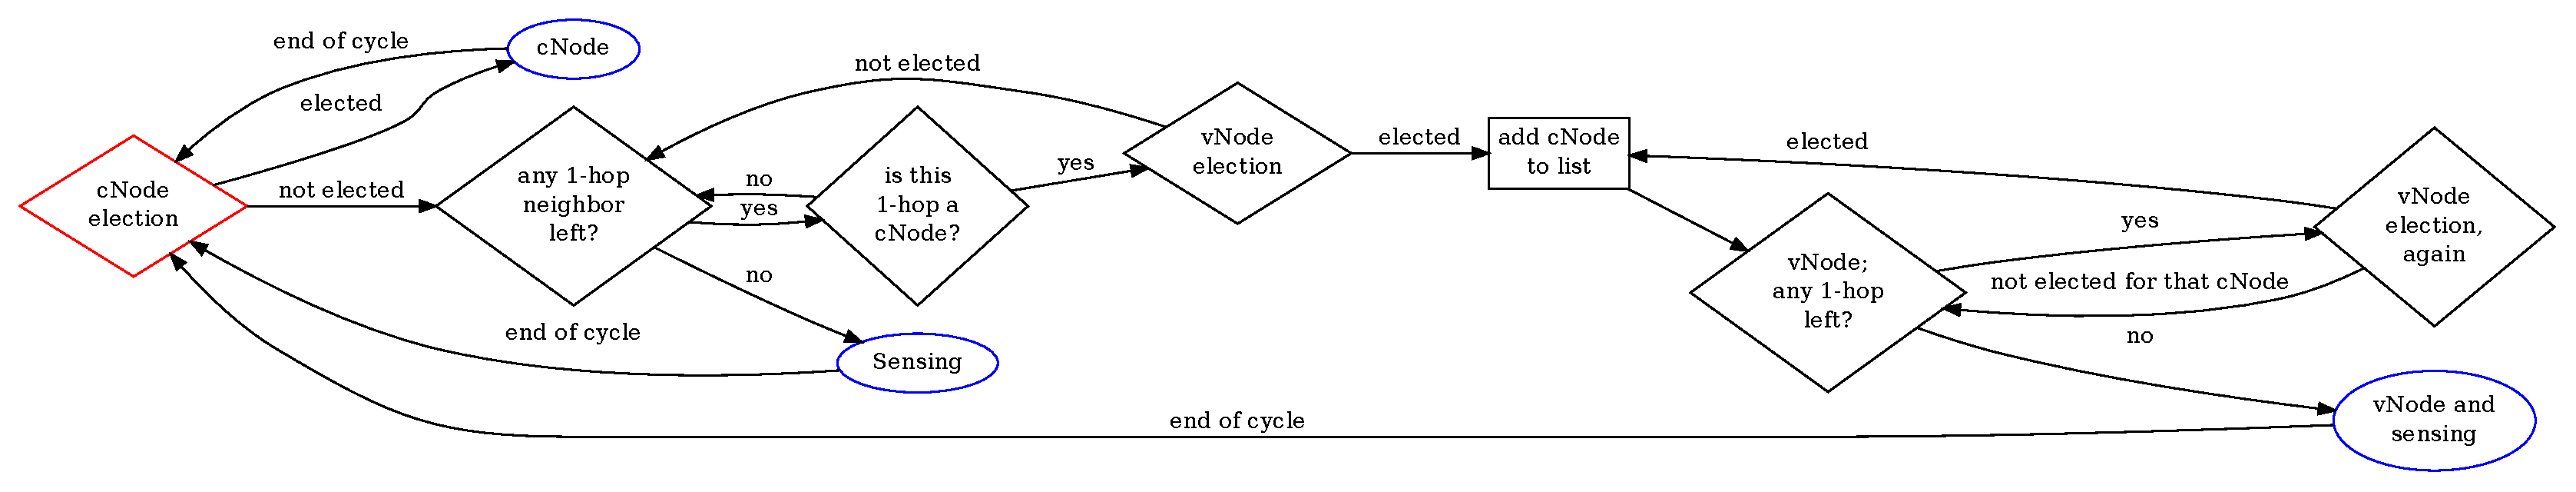
\includegraphics[width=\textwidth]{\chapterfig/state_graph.eps}
    \caption{State machine of the (non-\CH) nodes}\label{se:fig:states}
\end{figure*}

    \subsection{Cluster coverage in case of heterogeneous activity}

Deterministic election of the \cns does not only introduce a flaw that compromised nodes could try to exploit.
There is a second problem, independent from the nodes behavior, that could prevent the detection of compromised nodes.
If a region of the network happens to produce more traffic activity than the other parts of the network, the energy of its nodes will be drawn faster.
In consequence, none of the $n$ nodes with the highest residual energy ($n$ being the desired number of \cns during each cycle) will be located inside this region, and some nodes may not be covered for surveillance as long as traffic do not fade, possibly for all cycles.
\figurename~\ref{se:fig:cover} illustrates this problem.
\begin{figure}[h]
    \centering
    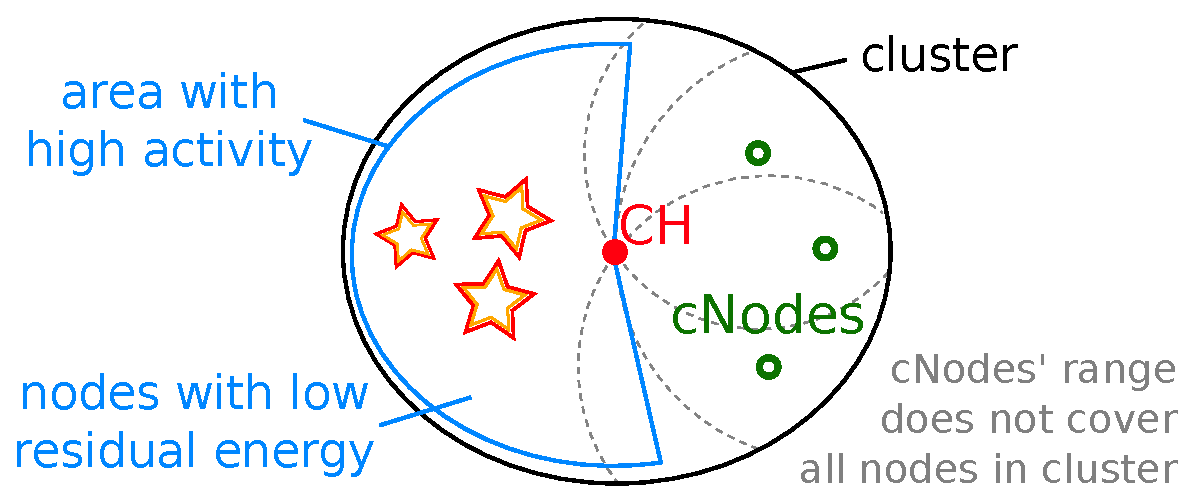
\includegraphics[width=.8\linewidth]{\chapterfig/cover.eps}
    \caption{Illustrative scheme: \cns are elected inside the area with less activity (thus with more residual energy) and do not cover nodes from the opposite side of the network.}\label{se:fig:cover}
\end{figure}

To address this issue we need to ensure that every node in the network is covered by at least one \cn.
So the election process we presented in~\ref{se:subsubsec:elec1} needs to be modified.
The correct version is as follows:

\begin{enumerate}
    \item During first step, each node evaluates its residual energy and broadcasts the value;
    \item The \ch listens to all values. Other nodes also register all messages they hear into memory;
    \item All nodes send to the \CH the list of their 1-hop neighbors\footnote{We do not deal with the case of compromised nodes cheating at this step of the process. Indeed they could announce extra virtual neighbors to try to escape from coverage.};
    \item The \CH picks the $n$ nodes among those with the highest residual energy, such that the $n$ nodes cover all other nodes in range\footnote{The details of the algorithm executed by the \ch at this step are not given in this study.}. If needed, it selects some additional nodes to cover all the cluster;
    \item The \CH returns to selected nodes a message to assign them the role of \cn.
\end{enumerate}

Note that some clustering algorithms (such as HEED~\cite{YF04} for example) provide other election mechanisms (for \chs, but that can also be used for selecting \cns) based on residual energy.
We do not want to use it because energy only takes part in the process as a factor for probability that the nodes declare themselves elected.
Instead we prefer nodes to broadcast their residual energy in order to enable surveillance by the \vns.

    \subsection{Observations}

\cns apply a very basic trust based scheme to the cluster: when a sensor node breaks a rule, for example by exceeding a given threshold for transmitted packets, it is considered as untrustworthy.
There are many other trust based schemes in literature, most of them more advanced than this one (see Section~\ref{se:sec:related}).
The \cns could implement several other trust mechanisms (by lowering a score on bad behaviour for each node for instance).
As more complex mechanism would create additional overhead, we prefer to limit to this simple method in this study.
%%%%%%%%%%%%%%%%%%%%%%%%%%%%%%%%%%%%%%%%%%%%%%%%%%%%%%%%%%%%%%%%%%%%%%%%%%%%%%%%%%%%%%
%%%%%%%%%%%%%%%%%%%%%%%%%%%%%%%%%%%%%%%%%%%%%%%%%%%%%%%%%%%%%%%%%%%%%%%%%%%%%%%%%%%%%%
%A first observation relates to overall complexity of the \cns election process.
%The proposed solution consists in the designation of nodes monitoring the monitors.
%The \vn role is a new role we introduce in the paper.
%It comes with a heavier election algorithm which make each node in the cluster send broadcast messages during the process (to announce residual energy and the list of direct neighbors).
%It is obvious that algorithmic complexity is increased, and that the system is heavier to implement than a simple pseudo-random election for the \cns.
%
%Along with overall complexity, overhead is also increased.
%Both those factors impact the nodes consumption.
%Note that we do not seek to decrease the comprehensive consumption of energy in the network; instead, we try to improve load balancing in order to keep alive as many nodes in the cluster as we can as time goes by.
%
%Another point not related to complexity is also worthy of interest: the use of \cns and \vns does not ensure a perfect guaranty of security.
%This system relies on several hypotheses, such as the fact that compromised nodes do not collaborate between them:
%a compromised node being elected as \cn could for instance announce to the \CH, during the election, that he can reach and survey some areas in the cluster, in order to make the \CH believe the area is surveyed (while in fact even the rogue \cn might not reach it).
%If the \CH does not assign other \cn to watch over this area, some other compromised nodes may go undetected and attack the network.
%
%The second hypothesis to note is that the proposed solution currently assumes that the \ch is not compromised.


\section{Selection in practice: results from simulation}
\label{se:sec:simul}

We have undertaken simulation of our proposal regarding the energy consumption in order to compare it with the previous model (using pseudo-random election for \cns).
We used \ns software to proceed.

In the new proposal, the \vns are to model the theoretical consumption of the \cns they watch over.
We have chosen to use Rakhmatov and Vrudhula's diffusion model\cite{RV01} to compute the consumption.
This choice was driven by several reasons:
\begin{itemize}
    \item it provides a pretty accurate approximation of real consumption, taking into account chemical processes internal to the battery such as rate capacity effect and recovery effect;
    \item it is one of the models already implemented in \ns. So in our case it is an absolutely perfect theoretical model.
        It remains ``theoretical'' as \vns use this model to compute the expected behaviour of \cns according to the few packets they sometimes hear. Meanwhile, real \cns consumption computed by \ns core takes into account every packet actually sent or received by \cns, also including packets that \vns can not hear (because of distance or sleep schedule). So the values computed by \vns and \ns core will not always be the same, which allows us to use the model.
\end{itemize}
Rakhmatov and Vrudhula's diffusion model refers to the chemical reaction happening inside the battery electrolyte, and is summarized by equation~(\ref{se:eqn:rvdm}).
\begin{equation}
    \label{se:eqn:rvdm}
    \sigma(t) = \underbrace{\int_{0}^{t} i(\tau) \, \mathrm d\tau}_{l(t)} \;+\; \overbrace{\int_{0}^{t} i(\tau) \left(2 \sum_{m=1}^{\infty} \exp^{-\beta^2 m^2 (t-r)} \right) \mathrm d\tau}^{u(t)}
\end{equation}
where:
\begin{itemize}
    \item $\sigma(t)$ is the apparent charge lost from the battery at $t$;
    \item $l(t)$ is the charge lost to the load (``useful'' charge);
    \item $u(t)$ is the unavailable charge (``lost in battery'' charge);
    \item $i(t)$ is the current at $t$;
    \item $\beta = \dfrac{\pi\sqrt{D}}{w}$, where $D$ is the diffusion constant and $w$ the full width of the electrolyte.
\end{itemize}
In practice, computing the first ten terms of the sum provides a good approximation (this is also the default behavior of \ns, by the way).

We launched several simulation instances and chose to focus on the energy consumption and load balancing in the cluster.
To obtain data about detection rate or false positive values of the \cns scheme, the reader is redirected to our previous work\cite{GMT12, BMM13}.
When we implemented our solution, we set the parameters of the simulation as detailed in Table~\ref{se:table:parameters}.

\begin{table}[ht]
    \centering
    \caption{Parameters used for simulations}
    \begin{tabular}{c c}
        \toprule
        Parameter & Value\\
        \midrule
        Number of nodes & 30 (plus 1~\CH)\\
        Number of \cns & 4\\
        Probability for \vns selection & 33~\%\\
        Delay between consecutive elections & 1~minute\\
        Simulation length & 30~minutes\\
        Cluster shape & Squared box\\
        Cluster length & Diagonal is 2$\times$50~meters\\
        Transmission range & 50~meters\\
        Location of the nodes & \CH: center; others: random\\
        Mobility of the nodes & Null\\
        Average data sent by normal nodes & 1024~bytes every 3~seconds\\
        Data sent by \vns (per target \cn) & 1024~bytes every 5~seconds\\
        \bottomrule
    \end{tabular}
    \label{se:table:parameters}
\end{table}

We obtained the residual energy values for each node at each minute of the simulation.
From this data we draw the average residual energy of the nodes (excluding \ch) as well as the standard deviation.
\begin{figure}[ht]
    \centering
    \includegraphics[width=.96\linewidth]{\chapterfig/mean.eps}
    \caption{Average residual energy of the nodes (excluding \ch)}\label{se:fig:mean}
\end{figure}
Average residual energy per minute in the batteries of the nodes is displayed on \figurename~\ref{se:fig:mean}.
Increasing values at $t=11$~minutes and $t=15$~minutes with the use of the proposed solution traduce the recovery effect of the batteries.
As expected, our proposal causes an increased global energy consumption.
This is due, of course, to the new \vn role.
\vns have to wake up periodically to send requests to neighbor \cns and to wait for an answer: this is energy-consuming.
The estimated overhead for our solution appears on \figurename~\ref{se:fig:overhead}.
\begin{figure}[ht]
    \centering
    \includegraphics[width=.96\linewidth]{\chapterfig/overhead.eps}
    \caption{Estimated number of generated packets during the simulation}\label{se:fig:overhead}
\end{figure}

%%%%%%%%%%%%%%%%%%%%%%%%%%%%%%%%%%%%%%%%%%%%%%%%%%%%%%%%%%%%%%%%%%%%%%%%%%%%%%%
%Along with overall complexity, overhead is also increased.
%Both those factors impact the nodes consumption.
%Note that we do not seek to decrease the comprehensive consumption of energy in the network; instead, we try to improve load balancing in order to keep alive as many nodes in the cluster as we can as time goes by.
Standard deviation of residual energy value in the nodes at each minute of the simulation is presented on \figurename~\ref{se:fig:stddev}.
\begin{figure}[ht]
    \centering
    \includegraphics[width=.96\linewidth]{\chapterfig/stddev.eps}
    \caption{Standard deviation for residual energy of the nodes}\label{se:fig:stddev}
\end{figure}
During the first minutes of simulation, our solution creates a higher disproportion in load balancing due to the introduction of \vns (there are more nodes assuming demanding functions).
But after the seven first minutes or so, the standard deviation with our method falls below the standard deviation of previous method.
This is the consequence of a better load repartition over the nodes with our solution.
The difference between standard deviation with and without our simulation may look small: this is due to the model of the simulation we implemented.
Given that we have a good pseudo-random numbers generator, when the number of elections get high, all nodes will roughly assume \cn role the same number of times in simulation \emph{not} using our solution.
As sensing nodes all have the same activity, a correct repartition of the \cn roles over the time leads to a good energy balance.
But in a situation where sensing nodes have different activity levels ---~for instance, if there is an area in the cluster when measured events occur much more often than in the other parts of the cluster~--- the consumption would not be equilibrated between all the nodes with the previous method; whereas our solution would deal well with this case, since \cns are elected according to residual energy.
Thus simulations show that the use of \vns leads to a higher energy consumption, but electing \cns on residual energy provides a better load repartition in the cluster.


\section{Conclusion}

\cns are used in clustered \wsns to monitor traffic of the nodes and to detect \dos attacks (\eg flooding, black hole attacks).
In this paper, we have proposed a new method to dynamically elect those \cns, based on their residual energy.
The aim of the proposed selection algorithm is to provide a better load balancing in the cluster.

We have addressed several issues related with the use of a deterministic selection.
Compromised nodes trying to systematically take over the \cn role are forced to abandon it for later cycle, or get detected, by \vns.
The \vn role is a new role we introduced to survey the \cns by matching their announced energy consumption with a theoretical model.
The issue of areas of the cluster uncovered by \cns, depending of the activity in the cluster, is addressed by enforcing covering of the whole cluster: the \ch is to designate additional \cns if needed.
Working with clusters ensures a good scalability of the solution.
It is also flexible, as \cns can endorse various trust-based model, and monitoring rules can be set to fight against several types of \dos attacks.
And the use of \vns is resilient to a small percentage of compromised \vns (depending on parameters set by user).

The results we have obtained through simulations show that even though using our simulation causes a higher global consumption of energy in the cluster, it provides a better load repartition between sensors.

Future works include improvements of our solution by adding monitoring of the \ch, as well as modeling a cluster with areas of different activity levels.
Also we would especially like to study the impact of the percentage of designated \vns on global energy consumption.


%===============================================================================
%===============================================================================
%   BIBLIOGRAPHIE
%===================
\bibliography{biblio,onrequest}
\bibliographystyle{IEEEtran} %unsrt %plain %alpha
%===============================================================================
\end{document}
